%
% $Id: karplus_strong.tex 14 2014-02-04 22:36:30Z nicb $
%
\svnInfo $Id: karplus_strong.tex 14 2014-02-04 22:36:30Z nicb $

\chapter{Filtri delle corde pizzicate}

Cosa succede se immetto un impulso unitario in un filtro comb?
Semplicemente, l'impulso torner\`a $L$ campioni dopo moltiplicato per il
coefficiente $R^L$.

Tutti gli altri campioni valgono $0$, per cui non succede niente tra il tempo
$0$ e il tempo $L$.

La risposta all'impulso sar\`a quindi:

% \begin{equation}
% 	h_t = \left \{ \begin{array}{l l l}
% 			R^t & & se t = 0 mod L\\
% 			0   & & per tutti gli altri campioni\\
% 	 \end{array}
% \end{equation}

Ossia $h_t = R^t$ per $t = 0,~L,~2L, \dots$ e $0$ altrimenti. Questa \`e una
sequenza periodica di impulsi alla frequenza fondamentale di $f_c / L~Hz$ -- una
frazione intera della frequenza di campionamento,
salvo il fatto che questi impulsi decadono con una velocit\`a determinata da $R$.
Pi\`u $R$ \`e vicino a 1, pi\`u lento sar\`a il decadimento, e viceversa.

Fin qui, nulla di particolarmente eccitante.
I suoni musicali, in particolare quelli percussivi,
sono caratterizzati da una variazione dello spettro nel tempo.
E` vero che in questo caso il suono decade nel tempo, ma il suo spettro
\emph{decade tutto insieme} e quindi non si modifica in maniera musicale.

Karplus e Strong suggerirono una modifica del filtro comb per poterlo rendere pi\`u musicale.
L'idea \`e semplicissima: si tratta di inserire un filtro passa--basso nel
loop di feedback in modo da attenuare pi\`u rapidamente le frequenze acute
rispetto a quelle gravi.

Il filtro passabasso pu\`o anche essere un semplicissimo filtro di media

\begin{equation}
				y_t = \nicefrac{1}{2} \left [ x_t + x_{t-1} \right ]
\end{equation}

con funzione di trasferimento

\begin{equation}\label{eqn: ks lop transfer function}
				H (z) = \nicefrac{1}{2} \left [ 1 + z^{-1} \right ]
\end{equation}

con uno zero che si trova in corrispondenza della frequenza di Nyquist,
poich\'e l\`i $z = -1$.
% Sostituendo $z = e^{i\omega}$ nell'eq.\ref{eqn: ks lop transfer function} avremo che
% 
% \begin{equation}\label{eqn: ks lop transfer function unit circle}
% 				H (\omega) = \nicefrac{1}{2} \left [ 1 + e^{-i\omega} \right ] = \nicefrac{1}{2} + \nicefrac{1}{2} e^{-i\omega}
% \end{equation}

\begin{figure}[htbp]
	\begin{center}
		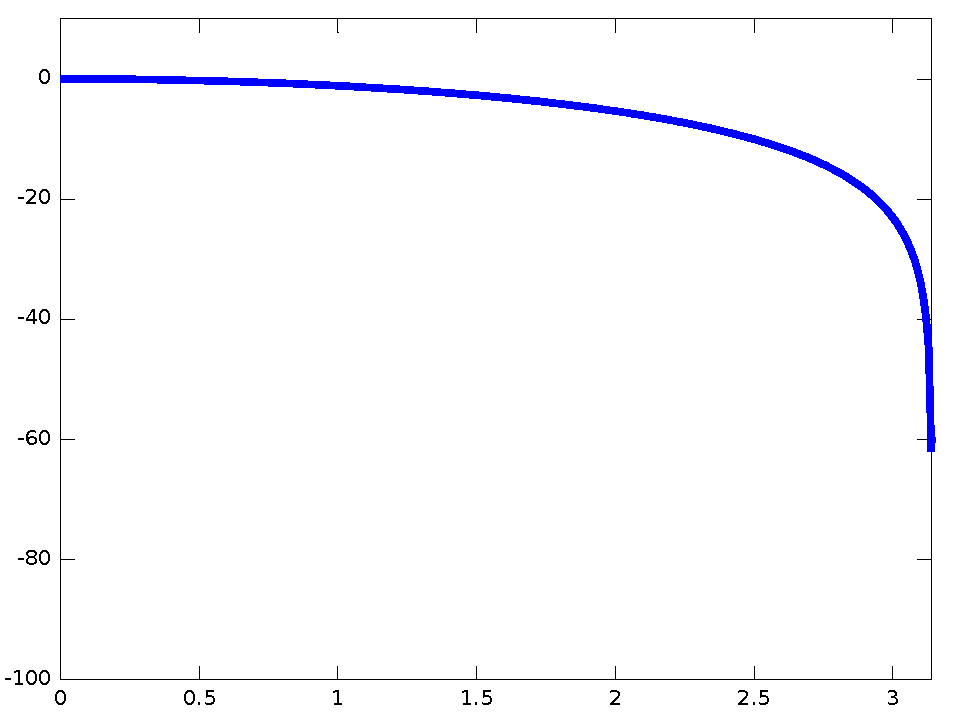
\includegraphics[width=0.75\textwidth]{\plotdir/ks_lop}
		\caption{La risposta in frequenza del filtro passabasso usato
		nell'algoritmo di Karplus e Strong\label{fig:ks lop frequency response}}
	\end{center}
\end{figure}

\subsection{Implementazione dei filtri delle corde pizzicate}

Per scrivere l'equazione del filtro,
\`e utile introdurre il segnale intermedio $w$,
il quale compare immedatamente dopo la chiusura del loop di feedback.
Il segnale $w$ \`e quindi determinato dall'ingresso $x$ e dal segnale di
output ritardato e pesato $y$:

\begin{equation}\label{eqn: ks first part}
				w_t = x_t + R^{L} y_{t-L}
\end{equation}

mentre l'uscita al tempo $t$ \`e determinata dal filtro FIR con input $w$,
quindi

\begin{equation}\label{eqn: ks second part}
				y_t = \nicefrac{1}{2} w_t + \nicefrac{1}{2} w_{t - 1}
\end{equation}

Quindi per ogni campione $t$ dobbiamo prima trovare $w_t$ nei termini
dell'equazione \ref{eqn: ks first part} e poi il valore dell'uscita $y_t$ da
$w_t$ e $w_{t - 1}$ secondo l'equazione \ref{eqn: ks second part}.

Cerchiamo ora di capire quale sia la risposta in frequenza di questo filtro.
Se guardiamo il segnale come vettore, le equazioni \ref{eqn: ks first part} e
\ref{eqn: ks second part} diventano

\begin{equation}\label{eqn: ks 1 ztransf}
		W = X + R^{L} z^{-L} Y
\end{equation}

\begin{equation}\label{eqn: ks 2 ztransf}
		Y = \nicefrac{1}{2} [ 1 + z^{-1} ] W
\end{equation}

Per trovare la funzione di trasferimento $H(z)$ dobbiamo risolvere l'equazione
per $Y / X$, ossia prima sostituire l'eq.\ref{eqn: ks 1 ztransf}
nell'eq.\ref{eqn: ks 2 ztransf} per ottenere solo $X$ e $Y$

\begin{equation}\label{eqn: ks X}
				X = 1 - R^L z^{-L} \nicefrac{1}{2} [ 1 + z^{-1} ]  
\end{equation}

e da qui trovare la funzione di trasferimento

\begin{equation}\label{eqn: ks transfer function}
				H ( z ) = Y / X = \frac{\nicefrac{1}{2} [ 1 + z^{-1} ]}{1 - R^{L} z^{-L} \nicefrac{1}{2} [ 1 + z^{-1} ]}
\end{equation}

Per risolvere questa equazione dobbiamo prima ottenere una formula pi\`u
chiara. Possiamo moltplicare numeratore e denominatore per $2 z^{L + 1}$:

\begin{equation}\label{eqn: ks transfer function 2}
				H ( z ) = Y / X = \frac{\nicefrac{1}{2} [ 1 + z^{-1} ] 2 z^{L+1}}{(1 - R^{L} z^{-L} \nicefrac{1}{2} [ 1 + z^{-1} ]) 2 z^{L + 1}} = \frac{z^{L + 1} + z^{L}}{2 z^{L+1} - R^{L} z - R^{L}}
\end{equation}

Per avere la risposta in frequenza dobbiamo valutare l'eq.\ref{eqn: ks transfer function 2}
sul cerchio unitario, quindi quando $z = e^{i \omega}$. Possiamo quindi
sostituire $z$ usando la formula di Eulero:

\begin{equation}
	\begin{array}{r c l}
		z & = & cos \omega + i sen \omega\\
		z^{L} & = & cos ( L \omega ) + i sen ( L \omega )\\
		z^{L+1} & = & cos ( (L + 1) \omega ) + i sen ( (L + 1) \omega )\\
	\end{array}
\end{equation}

Separando quindi le parti reali e le parti immaginarie dell'eq.\ref{eqn: ks
transfer function 2} sia al numeratore che al denominatore ottengo:

\begin{equation}\label{eqn: ks transfer function separated}
	\begin{array}{r c l}
		Reale ( numeratore ) & = & cos ( ( L + 1 ) \omega ) + cos ( L \omega )\\
		Immag ( numeratore ) & = & sin ( ( L + 1 ) \omega ) + sin ( L \omega )\\
		Reale ( denominatore ) & = & 2 cos ( ( L + 1 ) \omega ) - R^{L} cos \omega - R^{L} )\\
		Immag ( denominatore ) & = & 2 sin ( ( L + 1 ) \omega ) - R^{L} sin \omega )\\
	\end{array}
\end{equation}

A questo punto per trovare la risposta in frequenza devo trovare la
magnitudine di $H(z)$ sostituendo le equazioni \ref{eqn: ks transfer function separated}:

\begin{equation}\label{eqn: ks magnitude response}
				| H ( \omega ) | = \left [ \frac{[ Reale (numeratore) ]^{2} + [ Immag (numeratore) ]^{2}}{[ Reale (denominatore) ]^{2} + [ Immag (denominatore) ]^{2}} \right ]^{1/2}
\end{equation}

Realizziamone un'implementazione concreta per $L = 32$ con un coefficiente $R = 0.999$.
Dato che il ritardo totale del loop di feedback sar\`a di $32.5$ campioni,
ci aspettiamo che le risonanze siano ai multipli di $f_c / 32.5$.
